% IEEE conference-style project report. Compile with pdfLaTeX or XeLaTeX.
% Keep assets/ beside this file. No external .bib file is needed.
\documentclass[conference,letterpaper]{IEEEtran}
\usepackage[T1]{fontenc}
\usepackage[utf8]{inputenc}
\usepackage{cite}
\usepackage{graphicx}
\usepackage{booktabs}
\usepackage{tabularx}
\usepackage{array}
\usepackage{amsmath}
\usepackage{url}
\usepackage[hidelinks]{hyperref}
\graphicspath{{assets/}}
\newcolumntype{Y}{>{\raggedright\arraybackslash}X}
\newcolumntype{Z}{>{\centering\arraybackslash}X}
\setlength{\emergencystretch}{1.5em}

\title{Design and Verification of a Simplified Harvard Memory Organization}
\author{\IEEEauthorblockN{Yogesh Mishra (2401010518), Shagun Singh (2401010434)}
\IEEEauthorblockN{Pratyaksha Shastri (2401010348), Shiva Sharma (2401010441)}
\IEEEauthorblockN{Saksham Miglani (2401010401)}}
\begin{document}
\maketitle

\begin{abstract}
This project implements and verifies a simplified Harvard memory organization with independent instruction and data paths, and compares it with a single-port shared-memory baseline. The Harvard design contains separate 16-word instruction and data arrays, alignment and range decoding, and deterministic read/write control. A small controller executes ADDI, LW, SW, and a local EBREAK halt operation. The shared baseline contains one 32-word array and retains contending data requests for subsequent service. Eight self-checking testbenches complete 1,015 checks, and six Yosys synthesis runs report zero structural problems. A seven-instruction program retires in seven cycles and produces the expected result, x3 = 4. For one simultaneously requested instruction fetch and data read, Harvard completes both operations in one cycle, whereas the shared port requires two cycles. The result demonstrates port contention under the selected timing model; it does not establish a universal processor speedup or a maximum operating frequency.
\end{abstract}

\begin{IEEEkeywords}
Harvard architecture, shared memory, Verilog, address decoding, arbitration, simulation, memory organization.
\end{IEEEkeywords}

\section{Introduction}

Instruction fetching and data movement compete for memory resources when they share one service port. Separating the instruction and data paths creates an opportunity to perform both accesses within the same cycle. This project makes that difference observable using small register-transfer-level models rather than a complete processor or cache hierarchy.

The objective is to implement correct instruction/data separation, validate memory controls and timing, and compare behavior with a shared-memory organization. Deliverables include synthesizable Verilog RTL, block diagrams, an executable demonstration, self-checking simulations, VCD waveforms, and reproducible synthesis statistics. Both baseline organizations contain 1,024 bits of storage, enabling a controlled comparison of storage capacity while exposing their different interfaces and control overhead.

The main contribution is an explainable prototype in which architectural claims are tied to observable signals. Instruction validity, data validity, registered completion, pending-request state, and returned values are checked directly. The measured comparison is a two-operation contention experiment; the complete demonstration program is executed on the Harvard controller only.

\section{Literature Review}

\subsection{Stored Program and Harvard Organizations}

Von Neumann's EDVAC report provides foundational context for stored-program computing, describing memory and control within a general-purpose electronic computer \cite{ref1}. A stored-program organization should not be equated with an unavoidable single-port implementation: the port restriction is an explicit modeling choice in this project. The shared baseline therefore illustrates a memory-resource conflict rather than reproducing the full EDVAC architecture.

Microchip's AVR architecture documentation describes separate program/data memories and buses, permitting simultaneous program and data fetches \cite{ref2}. This is a practical example of the Harvard principle used here. AVR also uses pipelined execution, whereas the proposed prototype deliberately omits pipelining. Its instructional value comes from independent memory paths and visible arbitration, not from reproducing a commercial microcontroller.

\subsection{Instruction Semantics and Verification Tools}

The RV32I specification defines register arithmetic and a byte-addressed load/store model. ADDI uses a sign-extended immediate; LW and SW form effective addresses from a base register and signed offset. Register x0 is fixed at zero \cite{ref3}. These rules provide a familiar encoding for the demonstration controller. Only the required subset is implemented. The controller treats exact EBREAK as a local stop, instead of implementing the specification's debugging environment, and is not a compliant complete RISC-V core.

Icarus Verilog separates compilation/elaboration from simulation and supports testbenches that exercise intended hardware behavior \cite{ref4}. This supports the project's automated expected-value checks. GTKWave documents hierarchical signal selection and waveform display from simulation dumps \cite{ref5}; VCD files are therefore retained for interactive inspection as well as automated timing assertions. Neither waveform viewing nor a passing functional simulation establishes physical timing closure.

Yosys documents memory reads/writes as RTL cells and describes lowering memory into decoder and register logic \cite{ref6}. This distinction matters because a source-level array does not by itself guarantee a single read port or FPGA block-RAM implementation. The project explicitly checks read-port count before memory lowering and reports generic cell counts with their mapping limitations.

\subsection{Position of the Proposed Work}

The prototype combines these established ideas into a small teaching system. It isolates the effect of separate versus shared access paths, verifies request retention and address rejection, and supplies an executable load/store example. It does not propose a new processor architecture. Caches, coherence, virtual memory, interrupts, and physical SRAM delays remain outside its scope.

\section{Proposed Solution}

\subsection{Architecture and RTL Organization}

Fig.~\ref{fig:1} summarizes the two baseline organizations. The Harvard top connects instruction\_fetch, memory\_controller, and data\_memory. The fetch unit connects a 32-bit program\_counter to instruction\_memory. Both memories instantiate address\_decoder, preserving independent addresses and read outputs. Data requests are external inputs to the baseline top; a separate harvard\_demo module supplies instruction-controlled accesses using its own PC and register state.

\begin{figure}[!t]
\centering
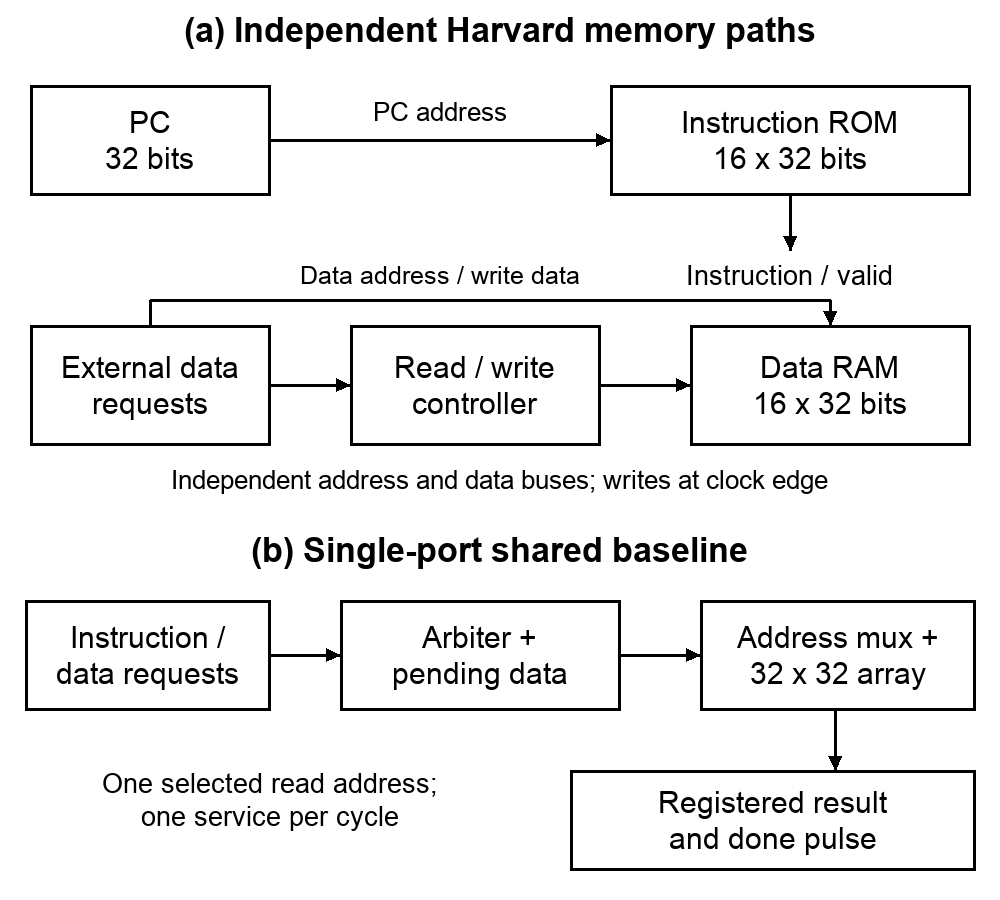
\includegraphics[width=\columnwidth]{memory_architecture.png}
\caption{Implemented memory organizations. Harvard has independent paths; the shared baseline selects one array address before reading.}
\label{fig:1}
\end{figure}

The instruction and data arrays each contain sixteen 32-bit words. Legal Harvard byte addresses are 0x00 through 0x3C in their respective address spaces. Sharing the same numerical address does not alias the arrays: a write at data address zero cannot modify instruction word zero. The default ROM contains deterministic instruction patterns, while DEMO\_PROGRAM = 1 selects the executable program without changing default-memory tests.

\begin{table}[!t]
\caption{Rtl Module Responsibilities}
\label{tab:I}
\centering\footnotesize
\renewcommand{\arraystretch}{1.15}
\setlength{\tabcolsep}{3pt}
\begin{tabularx}{\columnwidth}{Y Y}
\toprule
\textbf{Module} & \textbf{Responsibility} \\
\midrule
program\_counter & Reset to zero; advance by four \\
instruction\_memory & 16 x 32 ROM; valid fetch \\
instruction\_fetch & PC to instruction ROM \\
address\_decoder & Alignment and range checks \\
data\_memory & 16 x 32 RAM; edge writes \\
memory\_controller & Read/write gating and errors \\
harvard\_memory\_system & Separate baseline paths \\
shared\_port\_memory & One array; arbitration; retention \\
harvard\_demo & ADDI/LW/SW/stop execution \\
\bottomrule
\end{tabularx}
\end{table}

\subsection{Address Decoding and Read Write Control}

For address A, alignment requires A[1:0] = 00 and range validity requires A[31:6] = 0. The selected word is A[5:2]. Both conditions must hold before an array access is enabled. An invalid instruction address returns zero with instruction\_valid low; an invalid requested data access asserts access\_error and suppresses both read and write enables. This prevents high-bit or unaligned addresses from silently selecting a valid low-index word.

With no data request, the controller leaves both enables and the error output low. A valid read-only request enables a combinational read. A valid write request enables a write on the next rising edge. If read and write requests are asserted together, write priority suppresses the read. In the standalone RAM, a read held across an accepted write observes the old value before the edge and the new value after nonblocking updates settle.

Reset is synchronous and active high for sequential state. Arrays are initialized at time zero and are not cleared by reset. In the baseline Harvard top, reset affects the PC only, so an external requester must drive write requests idle to avoid writes during reset. The executable controller gates its own requests during reset, halt, or fault. Memory persistence and queued-request cancellation are tested explicitly.

\subsection{Single Port Shared Memory}

The shared array contains thirty-two 32-bit words. Instructions occupy byte addresses 0x00--0x3C and data occupies 0x40--0x7C. Both address regions require word alignment. This protection simplifies checking and is a restriction of the baseline, not a claim that all Von Neumann systems use separate protected regions.

At initial contention, a valid instruction request wins. The data address, write flag, and write payload are copied into pending registers. A pending data request is promoted on the following cycle even if an instruction request remains asserted. The captured payload, rather than changing live inputs, determines the delayed access. This ensures progress for a data request under the documented single-outstanding-request protocol.

An address multiplexer precedes one array read expression. Instruction/data service signals are mutually exclusive, and a selected store commits on a rising edge. Read results and done indications are registered. A requester holds its request until done, then deasserts it by the next rising edge. That requester is blocked during its completion cycle to prevent synchronous completion handling from replaying the operation. Invalid shared addresses are not acknowledged; a caller must validate addresses or use a timeout. Reset suppresses service and discards queued requests while preserving stored words.

\subsection{Executable Demonstration Controller}

The controller maintains thirty-two 32-bit registers, a PC, retirement count, halt flag, and fault flag. Each supported instruction retires at one rising edge. ADDI updates a destination register; LW consumes the combinational data result; SW uses synchronous RAM write control. Writes to x0 are suppressed. Unsupported instructions, invalid fetches, and invalid data requests set a sticky fault and stop execution. There are no branches or pipeline hazards in this straight-line subset.

\begin{table}[!t]
\caption{Executed Demonstration Program}
\label{tab:II}
\centering\footnotesize
\renewcommand{\arraystretch}{1.15}
\setlength{\tabcolsep}{3pt}
\begin{tabularx}{\columnwidth}{YZZ}
\toprule
\textbf{PC} & \textbf{Instruction} & \textbf{Effect} \\
\midrule
0x00 & addi x1, x0, 5 & x1 = 5 \\
0x04 & sw x1, 0(x0) & RAM[0] = 5 \\
0x08 & lw x2, 0(x0) & x2 = 5 \\
0x0C & addi x2, x2, -1 & x2 = 4 \\
0x10 & sw x2, 60(x0) & RAM[15] = 4 \\
0x14 & lw x3, 60(x0) & x3 = 4 \\
0x18 & ebreak & Local halt \\
\bottomrule
\end{tabularx}
\end{table}

The two stores and two loads exercise the first and last data words. During each load/store, the separate instruction path continues to supply the current instruction. This demonstrates overlapping instruction and data access in a single-cycle controller; it is not a claim of pipelined fetch of a future instruction. EBREAK is counted among the seven retired instructions and leaves the PC at 24.

\subsection{Verification and Reproducibility}

The latest full regression was executed on November 16, 2026, using Icarus Verilog 13.0 and Yosys 0.70+post. Testbenches use a 10 ns clock where applicable, four-state comparisons, and fatal termination on a mismatch. The regression requires a PASS marker, successful simulation, nonempty VCD output, and the generated performance report. A 256-transaction scoreboard uses seed 4127 and an independent expected-state array to check memory contents and rejected writes.

Waveform assertions parse timestamped VCD values to check concurrent Harvard validity, nonoverlapping shared service, the shared completion interval, measured cycle counters, and the program's halt/result state. Synthesis runs RTL and generic mapping flows for each of the two baselines and the demo controller. The RTL flow uses proc, opt, check -assert, and stat. The generic flow additionally runs memory and techmap, followed by optimization and structural checks. The shared RTL flow asserts exactly one \$memrd cell.

\section{Results And Discussion}

\subsection{Functional Verification}

All eight testbenches passed, totaling 1,015 checks (Table~\ref{tab:III}). These checks cover initialized contents, PC increments, byte-to-word decoding, read gating, synchronous writes, invalid-address rejection, and simultaneous access. Shared-memory checks additionally cover pending-write payload retention, request progress, completion turnaround, and reset cancellation. The executable-controller test also attempts an x0 write, an unsupported instruction, an unaligned load, and an out-of-range store.

\begin{table}[!t]
\caption{Functional Regression Results}
\label{tab:III}
\centering\footnotesize
\renewcommand{\arraystretch}{1.15}
\setlength{\tabcolsep}{3pt}
\begin{tabularx}{\columnwidth}{YZZ}
\toprule
\textbf{Testbench} & \textbf{Checks} & \textbf{Result} \\
\midrule
Program counter & 8 & PASS \\
Instruction memory & 38 & PASS \\
Data memory & 18 & PASS \\
Harvard integration & 36 & PASS \\
Shared port memory & 40 & PASS \\
Memory comparison & 14 & PASS \\
Executable demo & 36 & PASS \\
Memory edge cases & 825 & PASS \\
Total & 1015 & 8 / 8 PASS \\
\bottomrule
\end{tabularx}
\end{table}

The valid demonstration program retires seven instructions in seven cycles. Final registers are x1 = 5, x2 = 4, and x3 = 4. Data words zero and fifteen contain 5 and 4, respectively; halted is high, fault is low, and PC = 24. Halt prevents further retirement or data requests. A subsequent reset clears execution state while preserving RAM. These observations establish program-driven memory operation rather than instruction-pattern fetching alone.

\subsection{Measured Contention and Waveforms}

The comparison requests instruction address 0x04 and the first data word simultaneously. The instruction is 0x00100093; the data is 0x00000011. Both organizations must return these exact values before the workload is accepted as complete. For Harvard, values and valid signals are sampled at the consuming rising edge before the PC advances. Shared results are observed after their registered completions settle. Counters measure elapsed rising edges and are checked against expected counts only after completion.

\begin{figure}[!t]
\centering
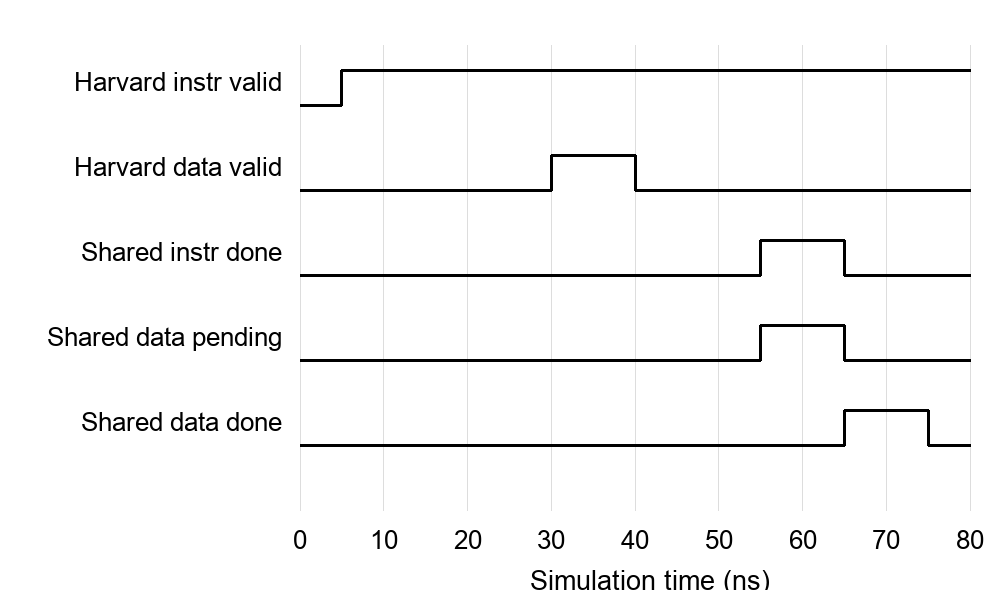
\includegraphics[width=\columnwidth]{comparison_waveform.png}
\caption{Actual comparison VCD transitions. Harvard is exercised at 30--40 ns; shared requests start at 50 ns and complete at 55 ns and 65 ns.}
\label{fig:2}
\end{figure}

\begin{table}[!t]
\caption{Simultaneous Two Operation Workload}
\label{tab:IV}
\centering\footnotesize
\renewcommand{\arraystretch}{1.15}
\setlength{\tabcolsep}{3pt}
\begin{tabularx}{\columnwidth}{YZZ}
\toprule
\textbf{Metric} & \textbf{Harvard} & \textbf{Shared} \\
\midrule
Completion cycles & 1 & 2 \\
Completed operations & 2 & 2 \\
Operations per cycle & 2.00 & 1.00 \\
Instruction result & 0x00100093 & 0x00100093 \\
Data result & 0x00000011 & 0x00000011 \\
\bottomrule
\end{tabularx}
\end{table}

The measured ratio is S = Cshared / CHarvard = 2 / 1 = 2.00. Throughput for the pair is Q = 2 / C, giving 2.00 and 1.00 operations/cycle. In the VCD, the shared instruction completion with pending data occurs at 55 ns, and data completion follows at 65 ns. Their 10 ns separation matches one test clock period. The plots use separate request windows for clarity; each workload counter begins at its own request event.

Harvard reads are combinational, whereas shared results are registered. Counting the first consuming edge for Harvard avoids treating a combinational output as a zero-cycle completion. Nevertheless, different interfaces and the shared requester's turnaround cycle mean this isolated pair is not a sustained streaming benchmark. The seven-instruction program is not run on the shared baseline, so no whole-program speedup is claimed.

\subsection{Synthesis and Resource Discussion}

All six synthesis runs report zero structural problems. The pre-lowering statistics confirm two independent Harvard read ports and one shared read port. Both baseline designs contain 1,024 memory bits. Table~\ref{tab:V} reports current baseline statistics; demo-controller resources are separate because its register file and execution logic would change the comparison scope.

\begin{table}[!t]
\caption{Baseline Synthesis Statistics}
\label{tab:V}
\centering\footnotesize
\renewcommand{\arraystretch}{1.15}
\setlength{\tabcolsep}{3pt}
\begin{tabularx}{\columnwidth}{YZZ}
\toprule
\textbf{Metric} & \textbf{Harvard} & \textbf{Shared} \\
\midrule
RTL arrays & 2 & 1 \\
RTL memory bits & 1024 & 1024 \\
RTL read ports & 2 & 1 \\
RTL cells & 59 & 95 \\
Generic cells & 1285 & 2513 \\
Generic multiplexers & 557 & 1219 \\
Generic sequential cells & 542 & 1128 \\
Structural problems & 0 & 0 \\
\bottomrule
\end{tabularx}
\end{table}

The shared design includes arbitration, captured-request state, and registered responses. Its array is also synthesized as writable storage logic, while the Harvard instruction ROM can be optimized from constants. The Harvard baseline includes a PC, which the shared memory-only baseline does not. These differences explain why the generic-cell totals are not an isolated measure of architectural area efficiency. They are Yosys internal cells, not FPGA LUTs, ASIC area, or power \cite{ref6}.

\subsection{Limitations and Future Evaluation}

The selected 10 ns test clock is a simulation stimulus, not a demonstrated 100 MHz hardware limit. No FPGA board test, target-specific memory inference, place-and-route analysis, setup/hold analysis, or maximum-frequency measurement was performed. Verilog initialization models power-up contents, but ASIC startup behavior and FPGA RAM initialization require a target implementation. Directed tests and a seeded scoreboard do not constitute exhaustive formal verification.

A next evaluation could select an FPGA, define clock constraints, implement a board interface, and validate reset and memory behavior in hardware. Matched registered interfaces, instruction-only/data-only workloads, sustained mixed streams, and identical executable programs on both systems would broaden the comparison. A shared lower-level memory or split caches would extend the study toward modified Harvard systems, but neither is required for the present prototype.

\section{Individual Contributions}

Table~\ref{tab:VI} records the assigned individual contributions. Pratyaksha Shastri and Saksham Miglani share responsibility for the executable controller and verification.

\begin{table}[!t]
\caption{Individual Contribution Record}
\label{tab:VI}
\centering\footnotesize
\renewcommand{\arraystretch}{1.15}
\setlength{\tabcolsep}{3pt}
\begin{tabularx}{\columnwidth}{Y Y}
\toprule
\textbf{Contributor and student ID} & \textbf{Assigned contribution} \\
\midrule
Shagun Singh\newline 2401010434 & Harvard memory RTL: program counter, instruction memory, instruction-fetch path, and top-level connections. \\
Yogesh Mishra\newline 2401010518 & Data memory and control: data RAM, address decoding, read/write control, alignment checks, and invalid-access handling. \\
Shiva Sharma\newline 2401010441 & Shared-memory implementation: single-port memory, arbitration, pending-request retention, and completion handshake. \\
Pratyaksha Shastri\newline 2401010348 & Executable controller and verification: demo program, controller, testbenches, simulation, and waveform analysis. \\
Saksham Miglani\newline 2401010401 & Executable controller and verification: demo program, controller, testbenches, simulation, and waveform analysis. \\
\bottomrule
\end{tabularx}
\end{table}

\section{Conclusion}

The project demonstrates a simplified Harvard memory organization with separate instruction and data paths, correct address/control behavior, and an executable load/store controller. Eight testbenches pass 1,015 checks, and all six synthesis runs pass structural checks. The executable program produces x3 = 4 after seven retired instructions. For the measured simultaneous fetch/read pair, the Harvard design completes in one cycle and the single-port baseline in two. This confirms that independent paths remove the modeled service-port conflict. The conclusion is limited to functional RTL and generic synthesis; hardware timing, physical resource efficiency, and broader workload performance remain future evaluation tasks.

\begin{thebibliography}{6}
\bibitem{ref1} J. von Neumann, First Draft of a Report on the EDVAC. Philadelphia, PA, USA: Moore School of Electrical Engineering, University of Pennsylvania, Jun. 1945. [Online]. Available: \url{https://web.mit.edu/STS.035/OldFiles/www/PDFs/edvac.pdf}
\bibitem{ref2} Microchip Technology Inc., ``AVR 8-bit Architecture,'' AVR42787: AVR Software User Guide AVR 8-bit Microcontrollers. Accessed: Nov. 16, 2026. [Online]. Available: \url{https://onlinedocs.microchip.com/oxy/GUID-78362176-487F-41B9-95C7-B478A9A186EB-en-US-2/GUID-58665E03-55DB-4291-ADAA-2E3A8C9CB261.html}
\bibitem{ref3} RISC-V International, ``RV32I Base Integer Instruction Set, Version 2.1,'' RISC-V Ratified Specifications Library, release v20260120. Accessed: Nov. 16, 2026. [Online]. Available: \url{https://docs.riscv.org/reference/isa/v20260120/unpriv/rv32.html}
\bibitem{ref4} Icarus Verilog Project, ``Simulation Using Icarus Verilog,'' Icarus Verilog documentation. Accessed: Nov. 16, 2026. [Online]. Available: \url{https://steveicarus.github.io/iverilog/usage/simulation.html}
\bibitem{ref5} GTKWave Authors, ``Launching GTKWave'' and ``Displaying Waveforms,'' GTKWave documentation. Accessed: Nov. 16, 2026. [Online]. Available: \url{https://gtkwave.github.io/gtkwave/quickstart/launching.html}
\bibitem{ref6} YosysHQ, ``Memory handling,'' Yosys documentation. Accessed: Nov. 16, 2026. [Online]. Available: \url{https://yosyshq.readthedocs.io/projects/yosys/en/latest/using_yosys/synthesis/memory.html}
\end{thebibliography}
\end{document}